\subsection{Архитектура программы}

Архитектура программы должна имитировать архитектуру конечного решения: то есть состоять из отдельных хранилищ, соединённых шиной для общения, а также присоединённого к ним мастера, через которого происходит управление системой. Общая схема представлена на рисунке \ref{fig:basic_architecture}.

\begin{figure}[h]
    \centering
    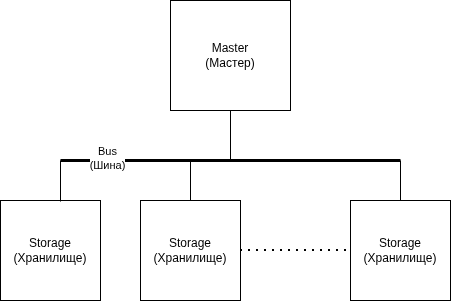
\includegraphics[width=0.6\textwidth]{extras/architeture.png}
    \caption{Общая схема архитектуры}
    \label{fig:basic_architecture}
\end{figure}

\subsection{Выбор алгоритмов}

Распределение данных в рамках разработанной системы выполняется в несколько последовательных этапов, формирующих полный цикл обработки графа в распределённой среде:

\begin{enumerate}
    \item вершины графа последовательно поступают в систему и распределяются по хранилищам с использованием алгоритма потокового распределения. На данном этапе формируется начальная конфигурация разбиения без учёта глобальной структуры графа;
    \item при достижении заранее заданного порогового значения количества добавленных вершин выполняется промежуточная процедура структурной оптимизации, направленная на локальное улучшение качества разбиения и уменьшение числа разрезанных рёбер;
    \item после завершения процесса первоначального добавления всех вершин выполняется дополнительный этап структурной оптимизации, который позволяет компенсировать накопленные локальные ошибки распределения и улучшить глобальное качество разбиения;
    \item после завершения фазы построения распределения начинается этап обработки запросов к графу. В ходе выполнения запросов производится поиск путей между вершинами с учётом текущего распределения данных по хранилищам;
    \item в процессе выполнения запросов осуществляется динамическая корректировка распределения данных, инициируемая вручную или по достижении заданных пороговых значений нагрузки. Данный этап позволяет адаптировать структуру распределения под изменяющийся профиль рабочей нагрузки.
\end{enumerate}

Таким образом, в рамках решаемой задачи необходимо использование четырёх ключевых алгоритмических компонентов:

\begin{itemize}
    \item алгоритма потокового распределения вершин;
    \item алгоритма структурной оптимизации разбиения графа;
    \item алгоритма структурной оптимизации с учётом динамической нагрузки;
    \item алгоритма поиска кратчайшего пути в графе.
\end{itemize}

\textbf{Алгоритм потокового распределения}

Для задачи потокового распределения и формирования начального разбиения графа был выбран алгоритм Fennel, подробно рассмотренный в разделе \ref{section:Fennel}. Основными причинами выбора данного алгоритма являются его низкая вычислительная сложность, линейная масштабируемость по числу вершин, а также способность обеспечивать балансировку нагрузки между хранилищами при минимизации числа разрезанных рёбер.

Дополнительно следует отметить, что качество начального разбиения, формируемого алгоритмом Fennel, оказывает существенное влияние на эффективность последующих этапов оптимизации, поскольку структурные алгоритмы работают с уже сформированным разбиением и улучшают его локальными перестановками.

\textbf{Алгоритм структурной оптимизации}

Для последующей оптимизации разбиения графа был выбран алгоритм Кернигана--Лина, описанный в разделах \ref{section:KL1} и \ref{section:KL2}. Данный алгоритм относится к классу итеративных методов локального улучшения разбиения и направлен на минимизацию стоимости разреза графа за счёт последовательного перемещения вершин между партициями.

Ключевым преимуществом алгоритма является возможность использования произвольной функции стоимости, что позволяет адаптировать его под специфику рассматриваемой системы. В данной работе в качестве целевой функции используется взвешенная стоимость разреза рёбер, учитывающая динамически изменяющуюся нагрузку.

\textbf{Учёт динамической нагрузки}

Для моделирования рабочей нагрузки используется подход, основанный на идеях системы Schism (раздел \ref{section:schism}). В рамках данной модели каждому ребру графа сопоставляется запросный вес:

\begin{equation*}
w_q(e),
\end{equation*}
который инициализируется значением:
\begin{equation*}
w_q(e) = 1.
\end{equation*}

В процессе выполнения запросов и построения маршрутов по графу веса рёбер динамически увеличиваются при каждом их использовании в найденных путях. Таким образом, формируется адаптивная модель нагрузки, отражающая реальную частоту обращения к различным участкам графа.

Данный механизм позволяет выделять «горячие» рёбра, которые чаще участвуют в запросах, и учитывать их с большей значимостью при последующей оптимизации распределения.

Алгоритм Кернигана--Лина использует данные веса при вычислении стоимости разбиения, что приводит к минимизации не просто количества разрезанных рёбер, а их суммарного веса. Это позволяет существенно повысить качество разбиения с точки зрения реальной рабочей нагрузки системы \cite{MetisOG}.

\textbf{Алгоритм поиска пути}

Для поиска кратчайшего пути в графе используется алгоритм A* \cite{AStar}. Выбор данного алгоритма обусловлен его эффективностью и широким распространением в задачах поиска путей в графовых структурах.

Алгоритм использует эвристическую оценку расстояния до целевой вершины, что позволяет существенно сократить пространство поиска по сравнению с классическими алгоритмами, такими как алгоритм Дейкстры. В рамках данной работы эвристика основана на геометрическом расстоянии между вершинами, что согласуется с моделью графа, в которой каждая вершина имеет координаты в двумерном пространстве.

Так как алгоритм A* является стандартным и хорошо изученным, его подробное рассмотрение выходит за рамки данной работы.

\subsubsection{Fennel алгоритм}

\begin{figure}[h]
    \centering
    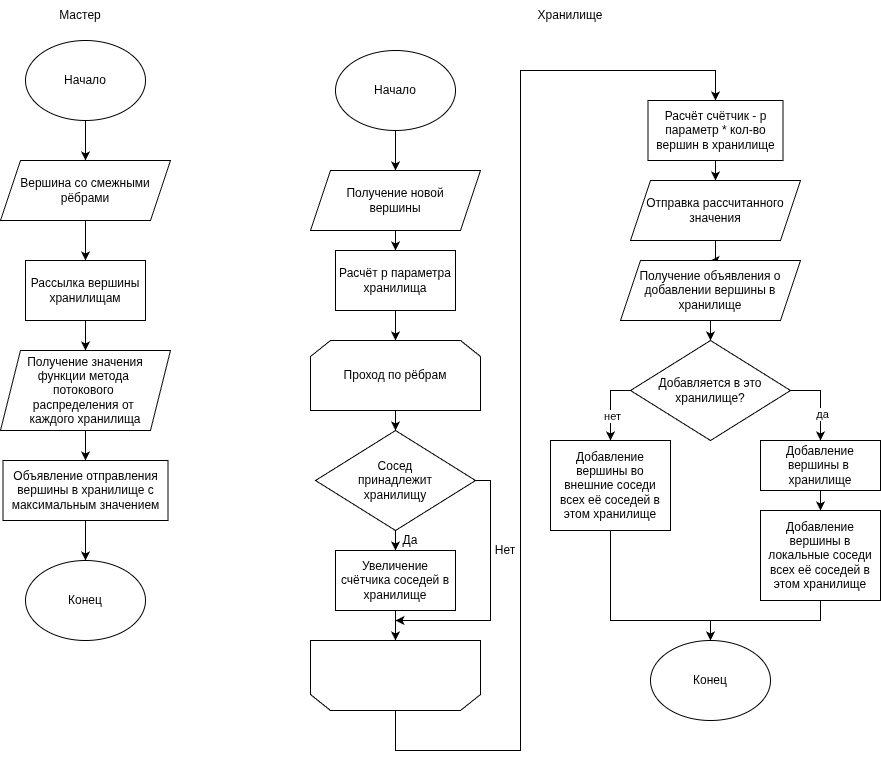
\includegraphics[width=\textwidth]{extras/contruction_part/Fennel.png}
    \caption{Схема распределения новой вершины в алгоритме Fennel}
    \label{project-fig:fennel}
\end{figure}

Реализация Fennel алгоритма, схема которой представлена на рисунке \ref{project-fig:fennel}, "вшивается" в хранилище, но часть действий происходит на мастере: Мастер отвечает за выбор хранилища для новой вершины, а каждое хранилище вычисляет локальную оценку размещения вершины.

\textbf{Работа мастера}

Работа алгоритма начинается с получения новой вершины вместе со списком её смежных рёбер. 
После этого мастер выполняет рассылку вершины всем хранилищам.

Каждое хранилище производит вычисление значения целевой функции и отправляет результат обратно мастеру. 
Мастер получает значения от всех хранилищ и выбирает хранилище с максимальным значением функции.

После выбора мастер рассылает уведомление о необходимости добавления вершины в выбранное хранилище.

\textbf{Работа хранилища}

После получения новой вершины хранилище начинает вычисление значения функции размещения.

Сначала вычисляется $p$ параметр хранилища, связанный с количеством вершин, уже находящихся в данном хранилище, нужный для балансировки. 
Затем выполняется проход по рёбрам вершины.

Для каждого соседа проверяется принадлежность текущему хранилищу. 
Если сосед уже размещён в данном хранилище, увеличивается счётчик локальных соседей

После завершения обхода рёбер вычисленное значение Fennel функции, которая использует $p$ параметр и счётчик соседей, отправляется мастеру.

\textbf{Добавление вершины}

После получения уведомления о размещении вершины хранилище проверяет, должна ли вершина быть добавлена локально.

Если вершина назначена данному хранилищу:
\begin{enumerate}
    \item вершина добавляется в хранилище;
    \item добавляются локальные соседи вершины;
    \item обновляются локальные связи.
\end{enumerate}

Если вершина назначена другому хранилищу, текущее хранилище сохраняет только внешние связи этой вершины для её соседей в этом хранилище.

После завершения операций обработка вершины считается завершённой.

\subsubsection{Алгоритм Кернигана-Лина}

\begin{figure}[h]
    \centering
    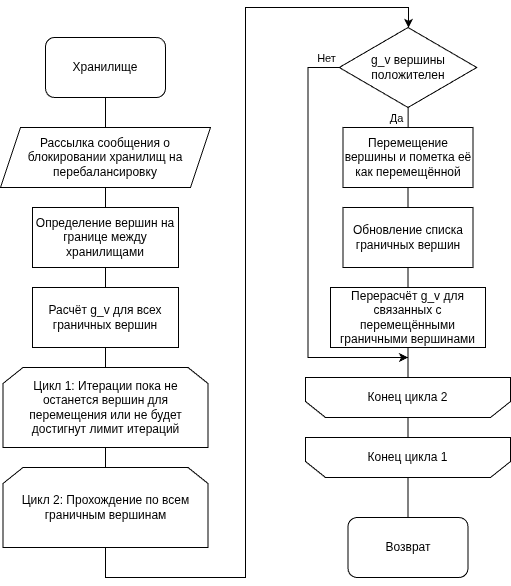
\includegraphics[height=0.6\textheight]{extras/contruction_part/KL.png}
    \caption{Схема уточнения распределения вершин алгоритмом Кернигана-Лина}
    \label{project-fig:KL}
\end{figure}

Реализация алгоритма Кернигана-Лина, схема которой представлена на рисунке \ref{project-fig:KL}, не вшивается в хранилище и является отдельным оптимизатором, работающим на мастере.

Алгоритм Кернигана--Лина используется для улучшения качества уже существующего разбиения графа между двумя хранилищами. 
Основная цель алгоритма заключается в уменьшении количества межхранилищных рёбер за счёт обмена вершинами между двумя хранилищами.

\textbf{Начало перебалансировки}

Перед началом выполнения алгоритма оба хранилища переводятся в режим перебалансировки. 
Для этого выполняется рассылка уведомлений о блокировке хранилищ, что предотвращает изменение структуры графа во время выполнения алгоритма.

После блокировки определяется множество граничных вершин. 
Граничными считаются вершины, имеющие связи с вершинами, расположенными в другом хранилище.

\textbf{Вычисление коэффициента перемещения}

Для каждой граничной вершины вычисляется значение $g_v$, характеризующее целесообразность её перемещения между хранилищами.

После вычисления значений начинается итерационный процесс перебалансировки. 


\textbf{Итерационный процесс}

Итерации продолжаются до тех пор, пока существуют вершины, которые могут быть перемещены, либо пока не будет достигнут лимит числа итераций.

Во время каждой итерации выполняется проход по всем граничным вершинам.
Для текущей вершины анализируется значение $g_v$:
\begin{enumerate}
    \item если значение положительно, вершина переносится в противоположное хранилище;
    \item после перемещения вершина помечается как уже обработанная;
    \item обновляется список граничных вершин;
    \item выполняется пересчёт значений $g_v$ для вершин, связанных с перемещённой вершиной.
\end{enumerate}

Если значение $g_v$ не является положительным, вершина остаётся в текущем хранилище.

\textbf{Обмен вершинами между хранилищами}

Так как алгоритм выполняется между двумя хранилищами, после принятия решения о перемещении вершины осуществляется обмен данными между узлами хранения.

Одно хранилище удаляет вершину из локального набора данных, а второе принимает вершину и добавляет её вместе с локальными связями. Так как обмен происходит объявлениями по шине, эти перемещения учитываются всеми хранилищами.
После завершения обмена обновляются сведения о принадлежности вершины и межхранилищных рёбрах.

\textbf{Завершение алгоритма}

После завершения всех итераций и отсутствия вершин, улучшающих текущее разбиение, алгоритм завершает работу.

Хранилища снимаются с режима блокировки и возвращаются в обычный режим обработки графа.

\subsubsection{Алгоритм выполнения запроса}

\begin{figure}[h]
    \centering
    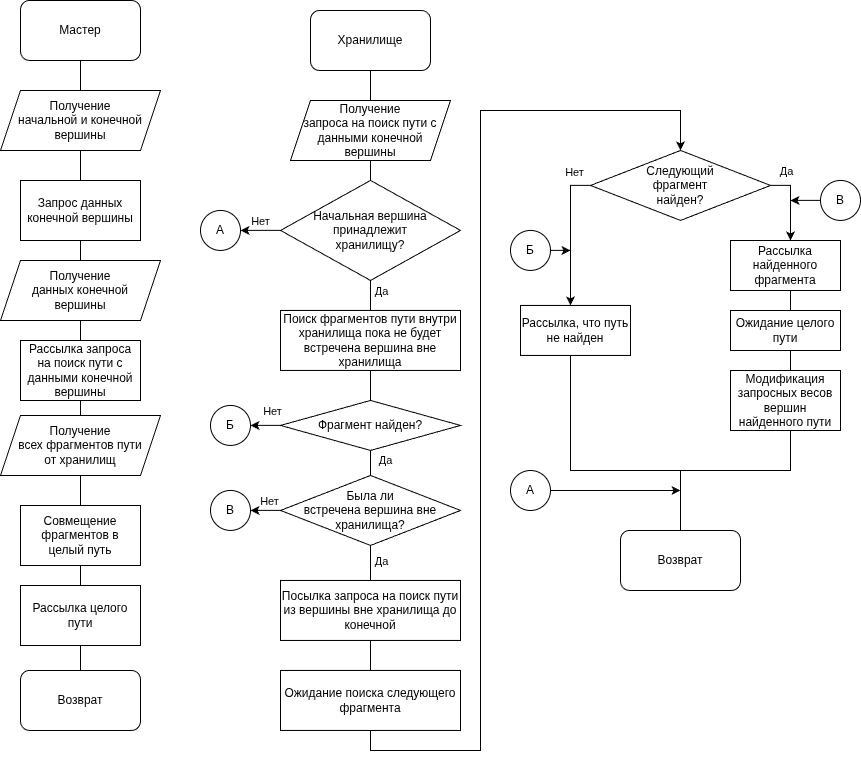
\includegraphics[width=\textwidth]{extras/contruction_part/request.png}
    \caption{Схема выполнения запроса на поиск пути}
    \label{project-fig:pathfinding}
\end{figure}

Реализация алгоритма, схема которой представлена на рисунке \ref{project-fig:pathfinding},  поиска пути распределена между мастером и хранилищами. Мастер отвечает за координацию процесса поиска и сбор найденных фрагментов пути, а хранилища выполняют локальный поиск пути в пределах своих данных и взаимодействуют друг с другом при переходе между областями хранения.

\textbf{Работа мастера}

Работа алгоритма начинается с получения начальной и конечной вершин пути.

После этого мастер запрашивает данные конечной вершины, необходимые для выполнения поиска пути. Получив информацию о конечной вершине, мастер формирует запрос на поиск пути и рассылает его всем хранилищам.

Каждое хранилище, которому принадлежит начальная вершина очередного фрагмента пути, выполняет локальный поиск и при необходимости передаёт поиск следующему хранилищу. В результате мастер получает найденные фрагменты пути от различных хранилищ.

После получения всех доступных фрагментов мастер выполняет их объединение в единый пути от начальной вершины до конечной.

Сформированный путь рассылается заинтересованным компонентам системы, после чего работа алгоритма завершается.

\textbf{Работа хранилища}

После получения запроса на поиск пути хранилище проверяет, принадлежит ли ему начальная вершина рассматриваемого фрагмента пути.

Если вершина не принадлежит данному хранилищу, запрос игнорируется. Если вершина находится в хранилище, начинается локальный поиск пути.

Поиск выполняется внутри данных хранилища до тех пор, пока не будет найдена конечная вершина либо вершина, принадлежащая другому хранилищу. Результатом поиска является фрагмент пути внутри текущего хранилища.

Если фрагмент genb не найден, хранилище формирует сообщение о невозможности продолжения поиска и завершает обработку запроса.

Если найденный фрагмент заканчивается вершиной, принадлежащей другому хранилищу, формируется новый запрос на поиск пути от этой вершины до конечной вершины. Запрос передаётся соответствующему хранилищу, после чего выполняется ожидание результата.

После получения следующего фрагмента пути хранилище передаёт найденный локальный фрагмент инициатору запроса. Если следующий фрагмент не найден, формируется сообщение об отсутствии полного пути между вершинами.

\textbf{Обработка найденного пути}

После формирования полного пути хранилище получает информацию о найденном пути и выполняет обновление локальных данных.

Для всех вершин, входящих в найденный путь:
\begin{enumerate}
    \item выполняется поиск соответствующих записей в хранилище;
    \item модифицируются веса вершин, принадлежащих найденному пути;
    \item обновлённые значения сохраняются в хранилище.
\end{enumerate}

После завершения обновления данных обработка genb считается завершённой.